\documentclass[12pt]{article}
\usepackage{graphicx} % Para imágenes
\usepackage[spanish]{babel} % Idioma del documento
\usepackage[colorlinks]{hyperref} % Para los enlaces
\usepackage{fancyhdr} % Para encabezados y pies de página
\usepackage{lastpage}
\usepackage{titlesec} % Control sobre los títulos
\usepackage{color} % Colores
\usepackage{geometry} % Margenes
\usepackage{afterpage}
\usepackage{setspace} % Espaciado entre lineas
\usepackage[dvipsnames]{xcolor}
\usepackage{xspace}
\hyphenpenalty=5000
\tolerance=1000
\usepackage{multicol}
\usepackage[toc,lof,lot]{multitoc}
\usepackage{subfig}
\usepackage{float}



\usepackage{fontspec}
\defaultfontfeatures{Renderer=Harfbuzz}
\setmainfont[
    ItalicFont=Labrada-Italic.ttf,
    BoldFont=Labrada-Variable.ttf,
    BoldItalicFont=Labrada-Italic.ttf,
    RawFeature={+axis={wght=400}},
    BoldFeatures={RawFeature={+axis={wght=700}}},
    BoldItalicFeatures={RawFeature={+axis={wght=700}}}
]{Labrada-Variable.ttf}

% Configuración de márgenes
\geometry{
 a4paper,
 left=25mm,
 right=25mm,
 top=20mm,
 bottom=20mm
}

% Configuración del enlace de colores
\hypersetup{
    linkcolor=tocColor,
    citecolor=Green,
    filecolor=Mulberry,
    urlcolor=NavyBlue,
    menucolor=BrickRed,
    runcolor=Mulberry,
    linkbordercolor=BrickRed,
    citebordercolor=Green,
    filebordercolor=Mulberry,
    urlbordercolor=NavyBlue,
    menubordercolor=BrickRed,
    runbordercolor=Mulberry
}

\newcommand\ruleafter[1]{#1\ \hrulefill}
\titleformat{\section}[hang]{\itshape\Large\bfseries\raggedright}{\thesection}{2pc}{\ruleafter}
\titlespacing*{\section}{0pt}{0pt}{8pt}

% Configuración de párrafos
\setlength{\parindent}{2.5em}
\setlength{\parskip}{1em} % Espaciado entre párrafos

% Encabezados y pies de página
\pagestyle{fancy}
\fancyhf{}
\fancyhead[L]{\color{textColor}\itshape Parte individual del proyecto del curso}
\fancyhead[R]{\color{textColor}\itshape Jesús Jiménez Montero}

\fancyfoot[L]{\color{textColor}\itshape\raggedright\parbox[t]{0.4\textwidth}{\leftmark}}
\fancyfoot[C]{\color{textColor}\hfill\makebox[0pt][c]{\hyperlink{toc}{\itshape Volver al Índice}}\hfill}
\fancyfoot[R]{\color{textColor}\itshape\hfill Página \thepage \xspace de \pageref*{LastPage}}

\setlength{\headheight}{14.5pt}
\renewcommand{\footrulewidth}{0.4pt}

% For subsections
\titleformat{\subsection}[hang]{\large\bfseries}{\thesubsection}{1em}{}\titlespacing*{\subsection}{1em}{*1}{*1}

% For subsubsections
\titleformat{\subsubsection}[hang]{\normalsize\bfseries}{\thesubsubsection}{1em}{}\titlespacing*{\subsubsection}{2.5em}{*1}{*1}

\definecolor{pageColor}{RGB}{250,248,245}
\definecolor{textColor}{RGB}{61, 61, 61}
\definecolor{tocColor}{RGB}{9, 138, 177}

\setlength{\marginparwidth}{2cm}

\renewcommand*{\multicolumntoc}{2}
\renewcommand*{\multicolumnlof}{2}
\renewcommand*{\multicolumnlot}{2}

%%%%%%%%%%%%%%%%%%%%%%%%%%%%%%%%%%%%%%%%%%%%%%%%%%%%%%%%%%%%%%%%%%%%%%%%%%%%%%%%%%%%%%%%%%%%%%%%%
\begin{document}
\pagecolor{pageColor}
\color{textColor}
% Portada
\begin{titlepage}
    \vspace*{\fill}

    \centering
    \parbox{0.8\textwidth}{    % Logo de la universidad
        
\includegraphics[width=0.7\textwidth]{imgs/marca-uji-color-fons-transparent.png}\par\vspace{1cm}

        {\Huge \bfseries \textit{Parte dividual del proyecto del curso} \par}
        {\Large \bfseries La Llama de Sant Antoni \par}

        % Información adicional
        \textsc{\large }
        \vspace{0.5cm} \\
        \textsc{\Large VJ1223 - \textit{Arte del Videojuego}}
        \vspace{0.5cm} \\
        \textsc{\large Año: 2024 - 2025}
        \vfill

        % Nombres de los autores
        \textbf{Realizado por:}         \\
        \href{https://www.richardotomislav.com/}{Jesús Jiménez Montero}      \\
    }
    \vspace*{\fill}
\end{titlepage}

% Índice de contenidos
%change the table of contents title
% \renewcommand{\contentsname}{Indice del documento}
\hypertarget{toc}{}
\tableofcontents
\newpage

\listoffigures
\newpage


\section{Introducción}
    En este documento, se presenta el arte que he realizado para \textit{La Llama de Sant Antoni}. Un detalle a mencionar es que, he tomado principalmente el rol de programador durante la creación de este videojuego, por lo tanto, tuve un rol algo menor en cuanto a la creación del arte. Me centré en crear bases de arte para que luego el artista del grupo, Lucas Godoy Nebot, pudiese revisarlo y adaptarlo al estilo del juego.

\section{Arte de personaje / Remedios}
    Tuve la tarea de diseñar uno de los personajes principales para el juego.

    Este personaje es la novia de Zacarías, el personaje principal.
    \subsection{Concepto}
        Probé con varias poses calcando de un modelo 3D para poder tener una idea de cómo se vería el personaje en el juego. Luego de varias pruebas, se decidió que la pose de la figura \ref{fig:remedios} era la que mejor se adaptaba al juego.

        \begin{figure}[H]
            \centering
            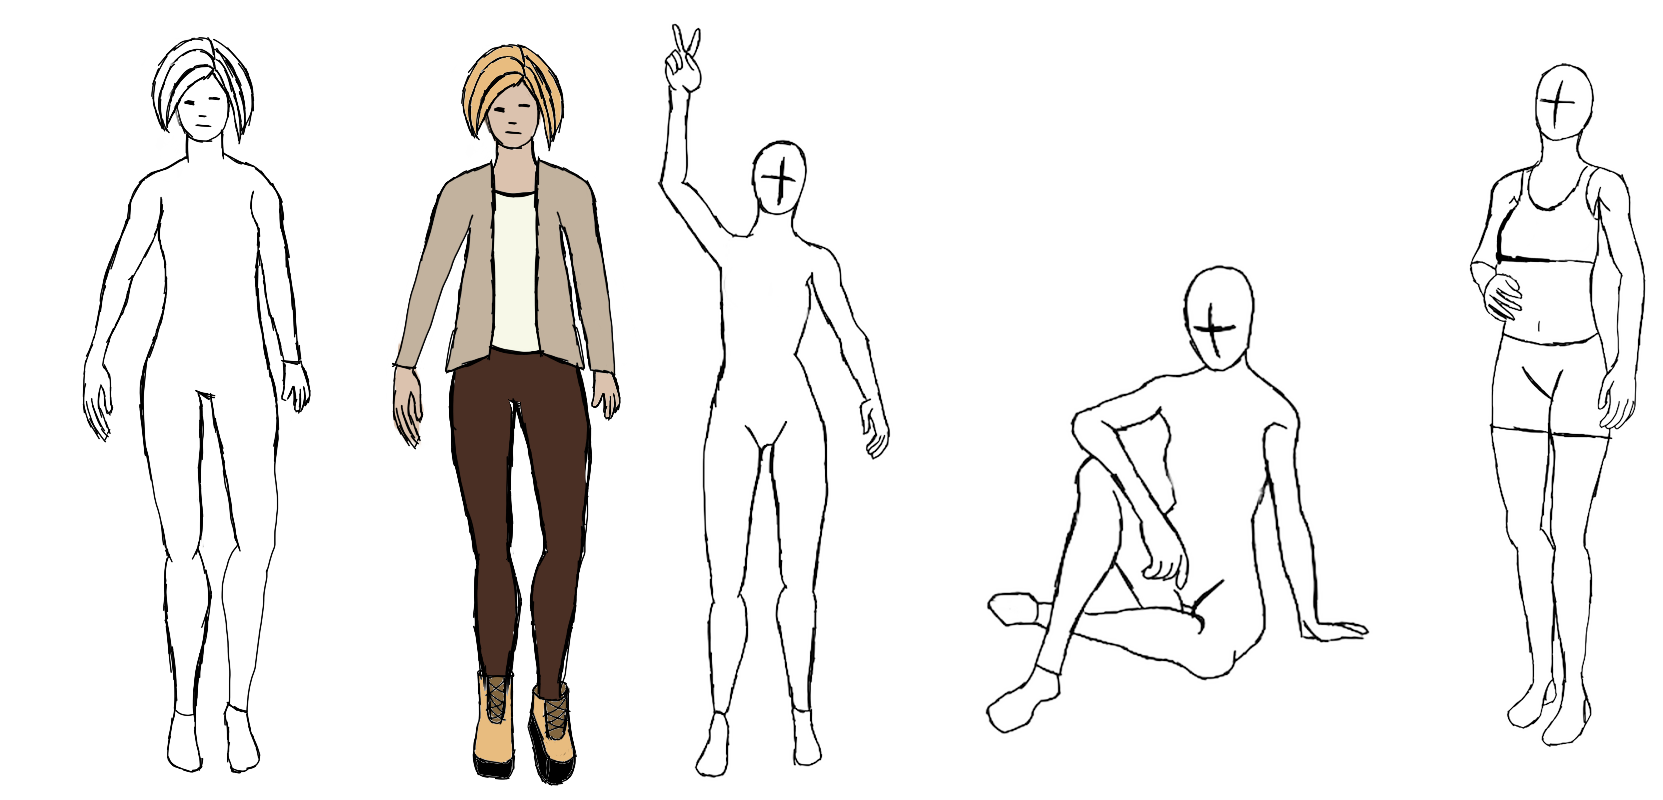
\includegraphics[width=\textwidth]{imgs/remedios_libro_arte.png}
            \caption{Bocetos conceptuales de Remedios}
            \label{fig:remedios}
        \end{figure}

    \newpage
    \subsection{Versión final}
        Decidí que la versión final quería que tuviese un libro en la mano, para darle un toque más intelectual a Remedios.

        \begin{figure}[H]
            \centering
            \begin{minipage}{.4\textwidth}
                \subfloat[Boceto final de Remedios, antes de la revisión]{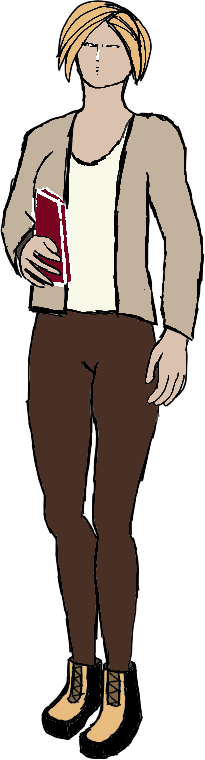
\includegraphics[width=0.8\textwidth]{imgs/rem_pre.PNG}\label{fig:sub_a}}
            \end{minipage}
            \hfill
            \begin{minipage}{.4\textwidth}
                \subfloat[Boceto revisado por mí, antes de la revisión de Lucas]{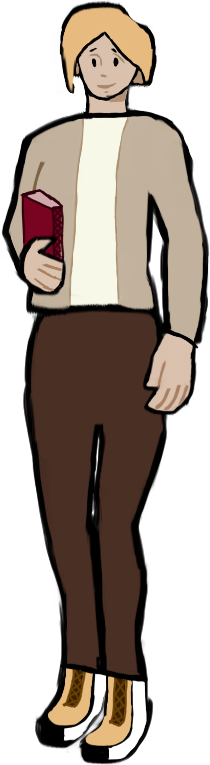
\includegraphics[width=0.8\textwidth]{imgs/remedios_final.PNG}\label{fig:sub_b}}
            \end{minipage}
                % \caption{Combined figure}\label{fig:sub}
        \end{figure}

    \newpage
    \subsection{Versión revisada}
        Esta la versión del personaje revisada por Lucas.
        \begin{figure}[H]
            \centering
            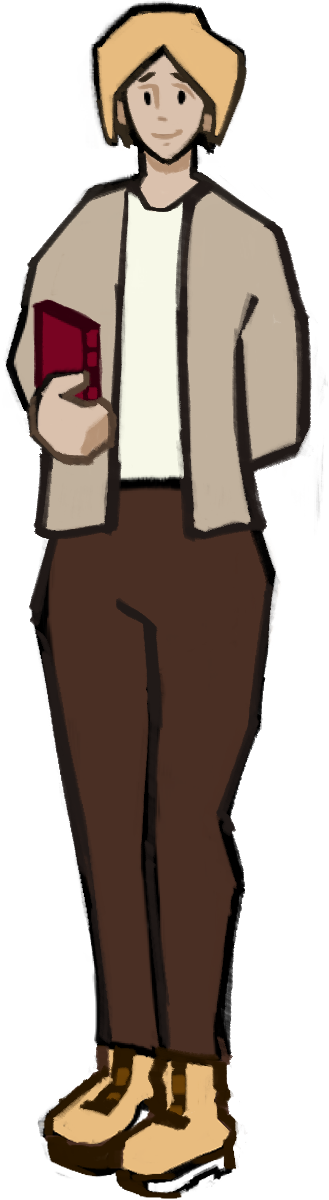
\includegraphics[height=0.8\textheight]{imgs/Remedios.png}
            \caption{Versión revisada de Remedios, por Lucas}
            \label{fig:remedios_final}
        \end{figure}

\newpage
\section{Arte de las calles}

    \subsection{Inicios}
        Al inicio, no teníamos muy claro como se iba a ver el juego ni qué estilo usar. Decidí hacer un boceto por mi cuenta tomando de referencia algunas ideas que ya teníamos para el estilo.
        No nos terminó de convencer el estilo tan sucio, pero no obstante, tomamos cierta inspiración de como se tenían que ver las calles dibujadas.

        \begin{figure}[H]
            \centering
            \begin{minipage}[b]{0.45\textwidth}
                \centering
                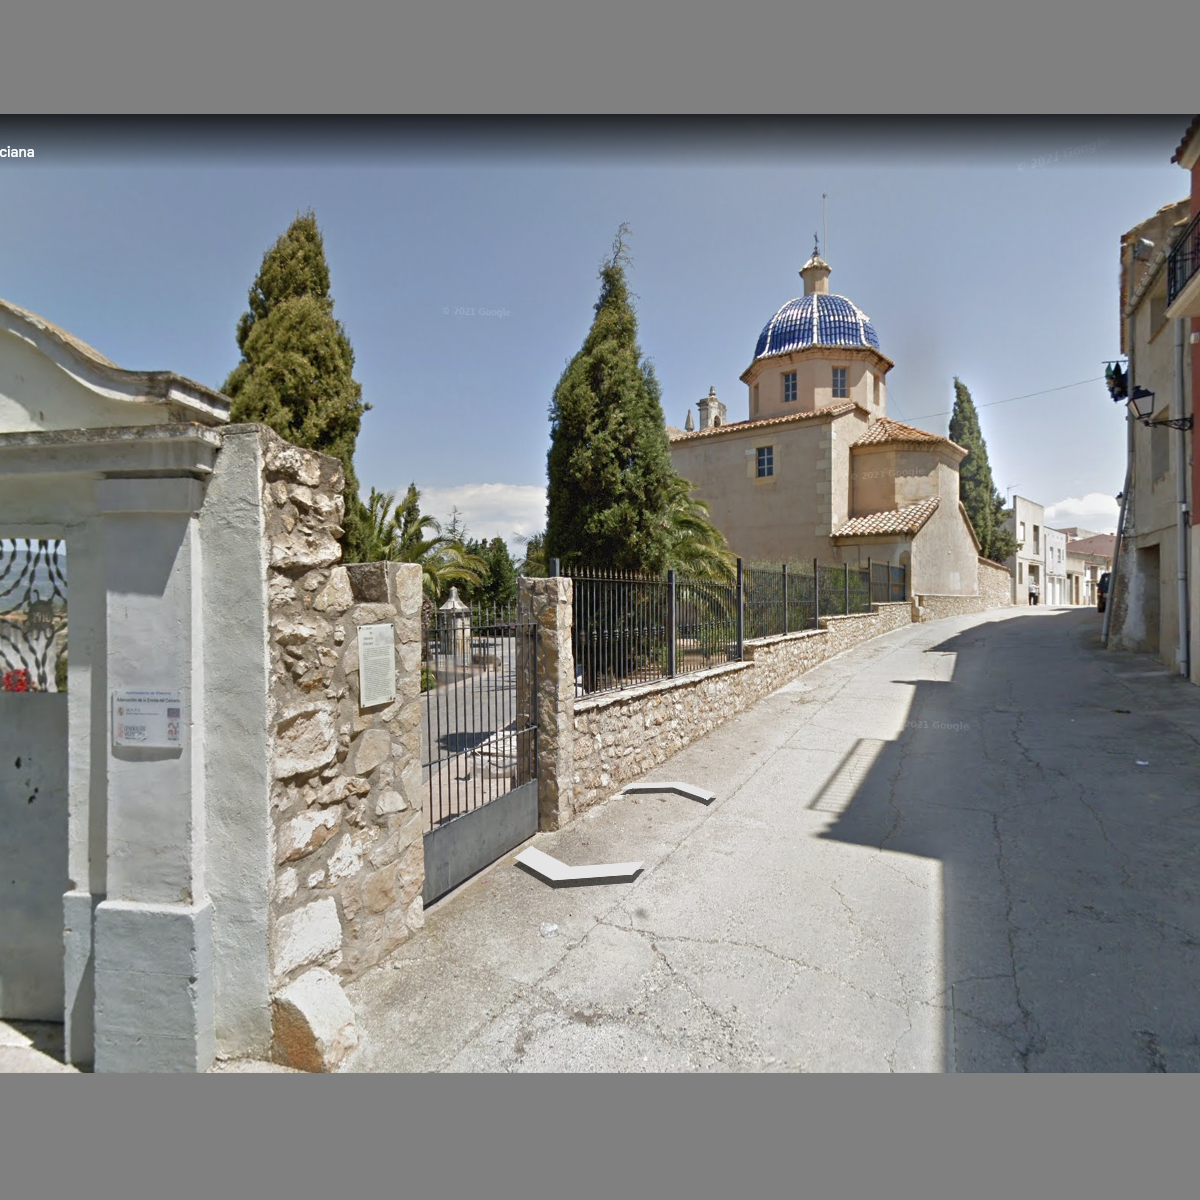
\includegraphics[width=\textwidth]{imgs/escenario_minijuego_foto.png}
                \caption{Boceto de las calles - Foto}
                \label{fig:calle_boceto_foto}
            \end{minipage}
            \hspace{0.05\textwidth}
            \begin{minipage}[b]{0.45\textwidth}
                \centering
                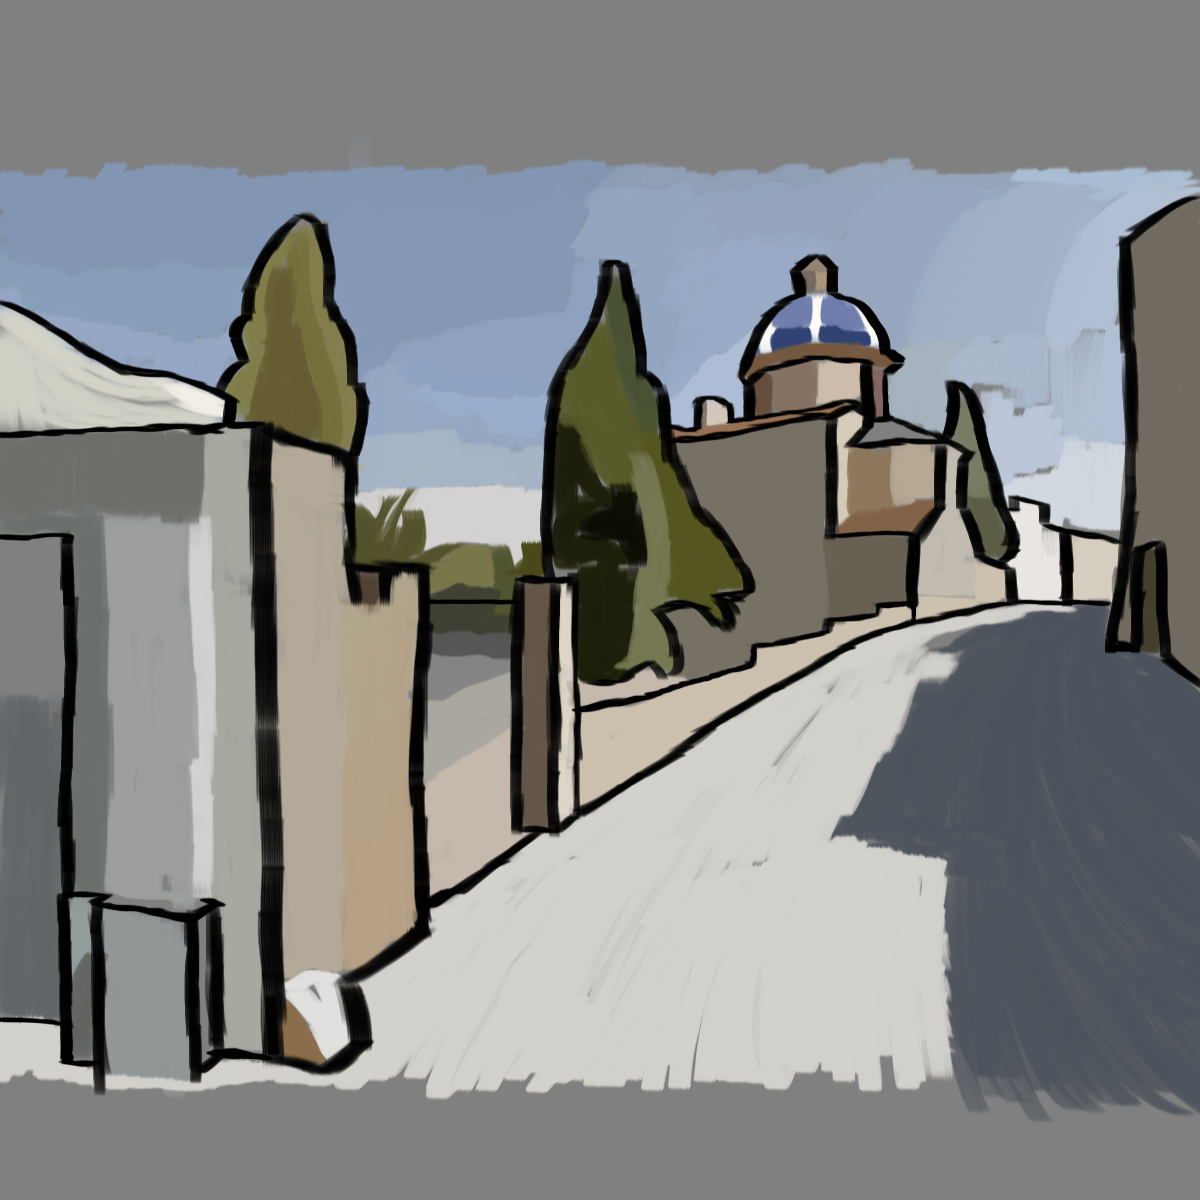
\includegraphics[width=\textwidth]{imgs/escenario_minijuego.png}
                \caption{Boceto de las calles - Dibujo}
                \label{fig:calle_boceto_dibujo}
            \end{minipage}
        \end{figure}
    \subsection{Después de decidir el estilo artístico}
    Una parte muy importante para mi minijuego era el dibujado y representación de las calles de Sant Antoni. Para ello, tomamos fotografías de las calles a nivel del ojo para que pareciese que el jugador estuviese viendo las calles.\\
    Después, dibujamos encima de ellas respetando la estructura de la calle; y otorgando más detalle al primer plano y según se llegaba al fondo de la fotografía, los edificios se convertían en bloques de color.\\
    \textbf{NOTA:} Para simplificar el documento, se omiten las versiones revisadas de los dibujos. Estas se pueden ver en el documento de Lucas.

    % Add new content here
    % En las figuras anteriores podemos ver el proceso de trabajo realizado en la Calle Torre.
    \begin{itemize}
        \item Las figuras \ref{fig:torre_foto_1} y \ref{fig:torre_boceto_1} muestran la primera sección de la calle y su interpretación artística.
        \item Las figuras \ref{fig:torre_foto_2} y \ref{fig:torre_boceto_2} representan la siguiente sección.
        \item Las figuras \ref{fig:torre_foto_3} y \ref{fig:torre_boceto_3} ilustran la tercera parte de la calle.
        \item Las figuras \ref{fig:torre_foto_4} y \ref{fig:torre_boceto_4} muestran la última sección de la Calle Torre.
    \end{itemize}

    \clearpage
    \subsection{C/Torre}
    % Update C/Torre figure labels
    \begin{figure}[h!]
        \centering
        \includegraphics[width=\textwidth]{imgs/C_torre_foto_0.JPG}
        \caption{Calle Torre: Fotografía de la primera sección}
        \label{fig:torre_foto_1}
    \end{figure}

    \begin{figure}[h!]
        \centering
        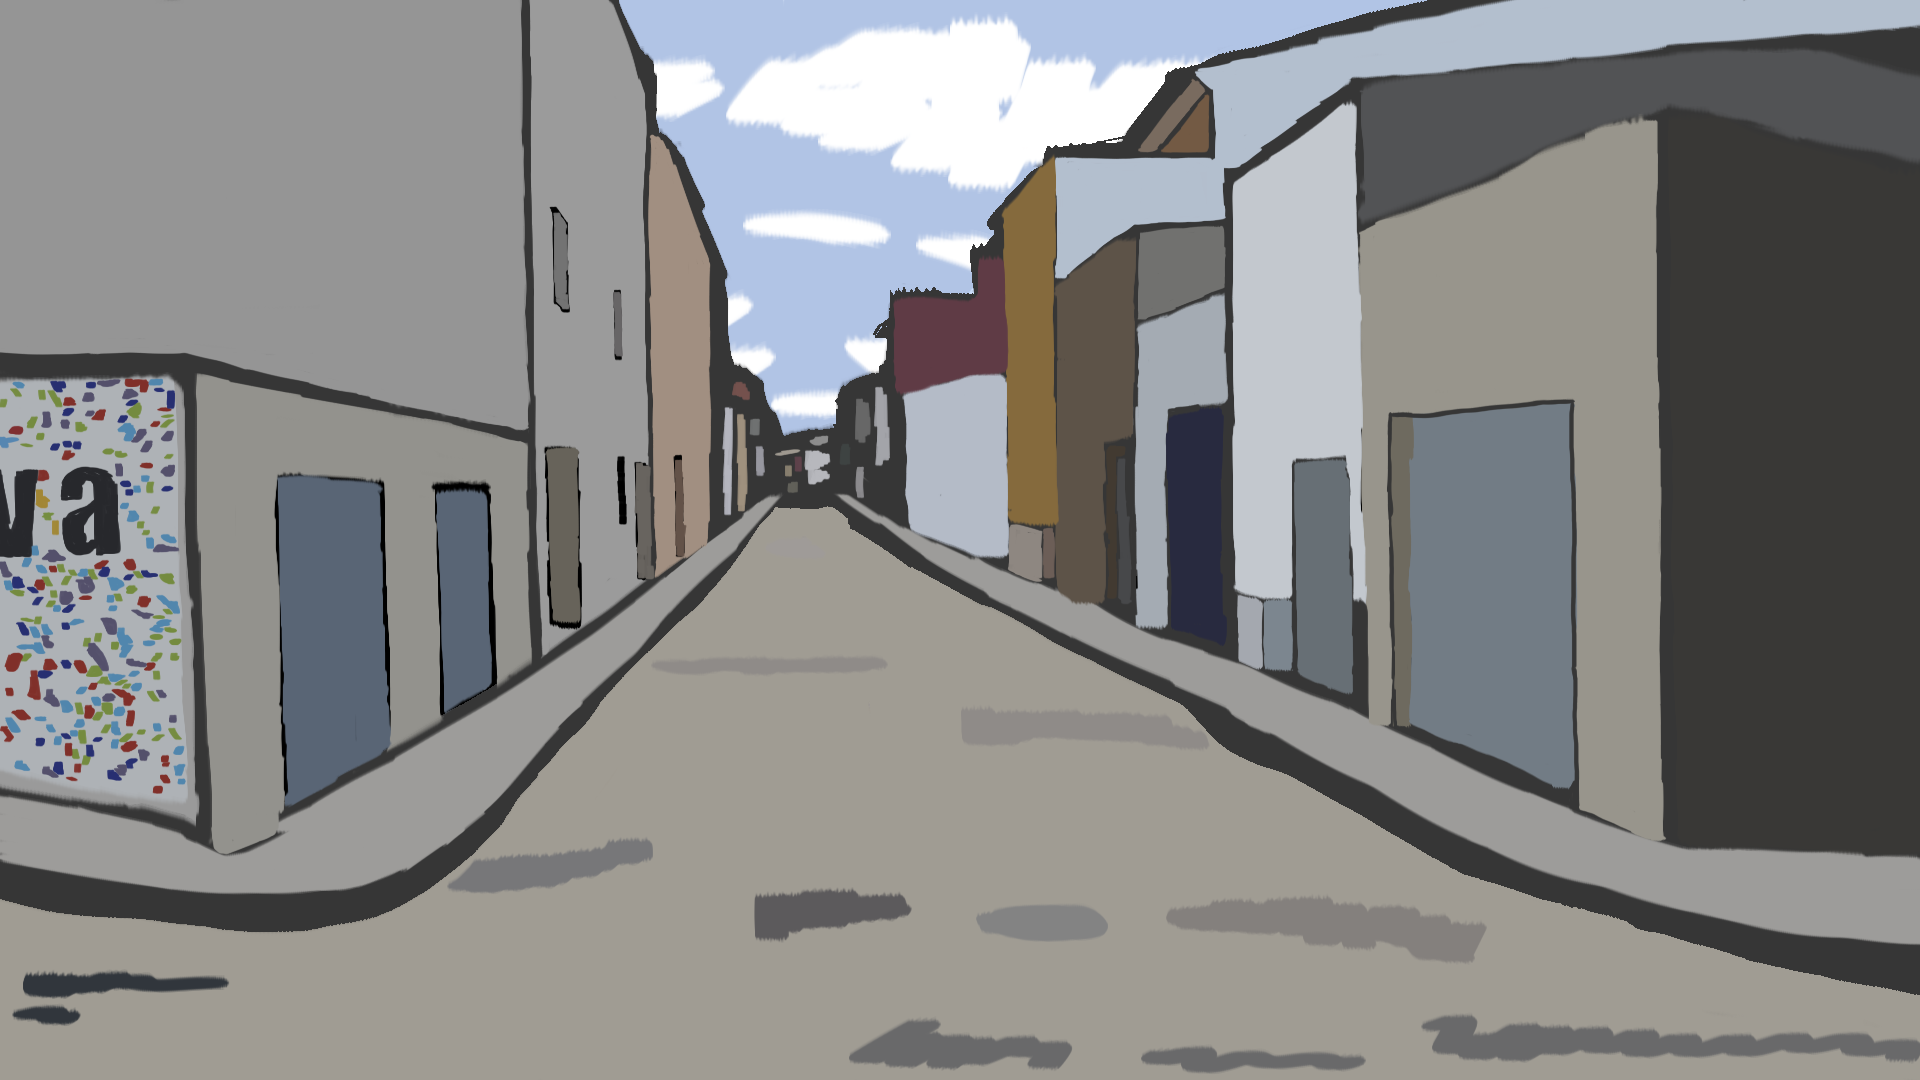
\includegraphics[width=\textwidth]{imgs/c_torre_1.png}
        \caption{Calle Torre: Boceto de la primera sección}
        \label{fig:torre_boceto_1}
    \end{figure}
    \clearpage
    \begin{figure}[h!]
        \centering
        \includegraphics[width=\textwidth]{imgs/C_torre_foto_1.JPG}
        \caption{Calle Torre: Fotografía de la segunda sección}
        \label{fig:torre_foto_2}
    \end{figure}

    \begin{figure}[h!]
        \centering
        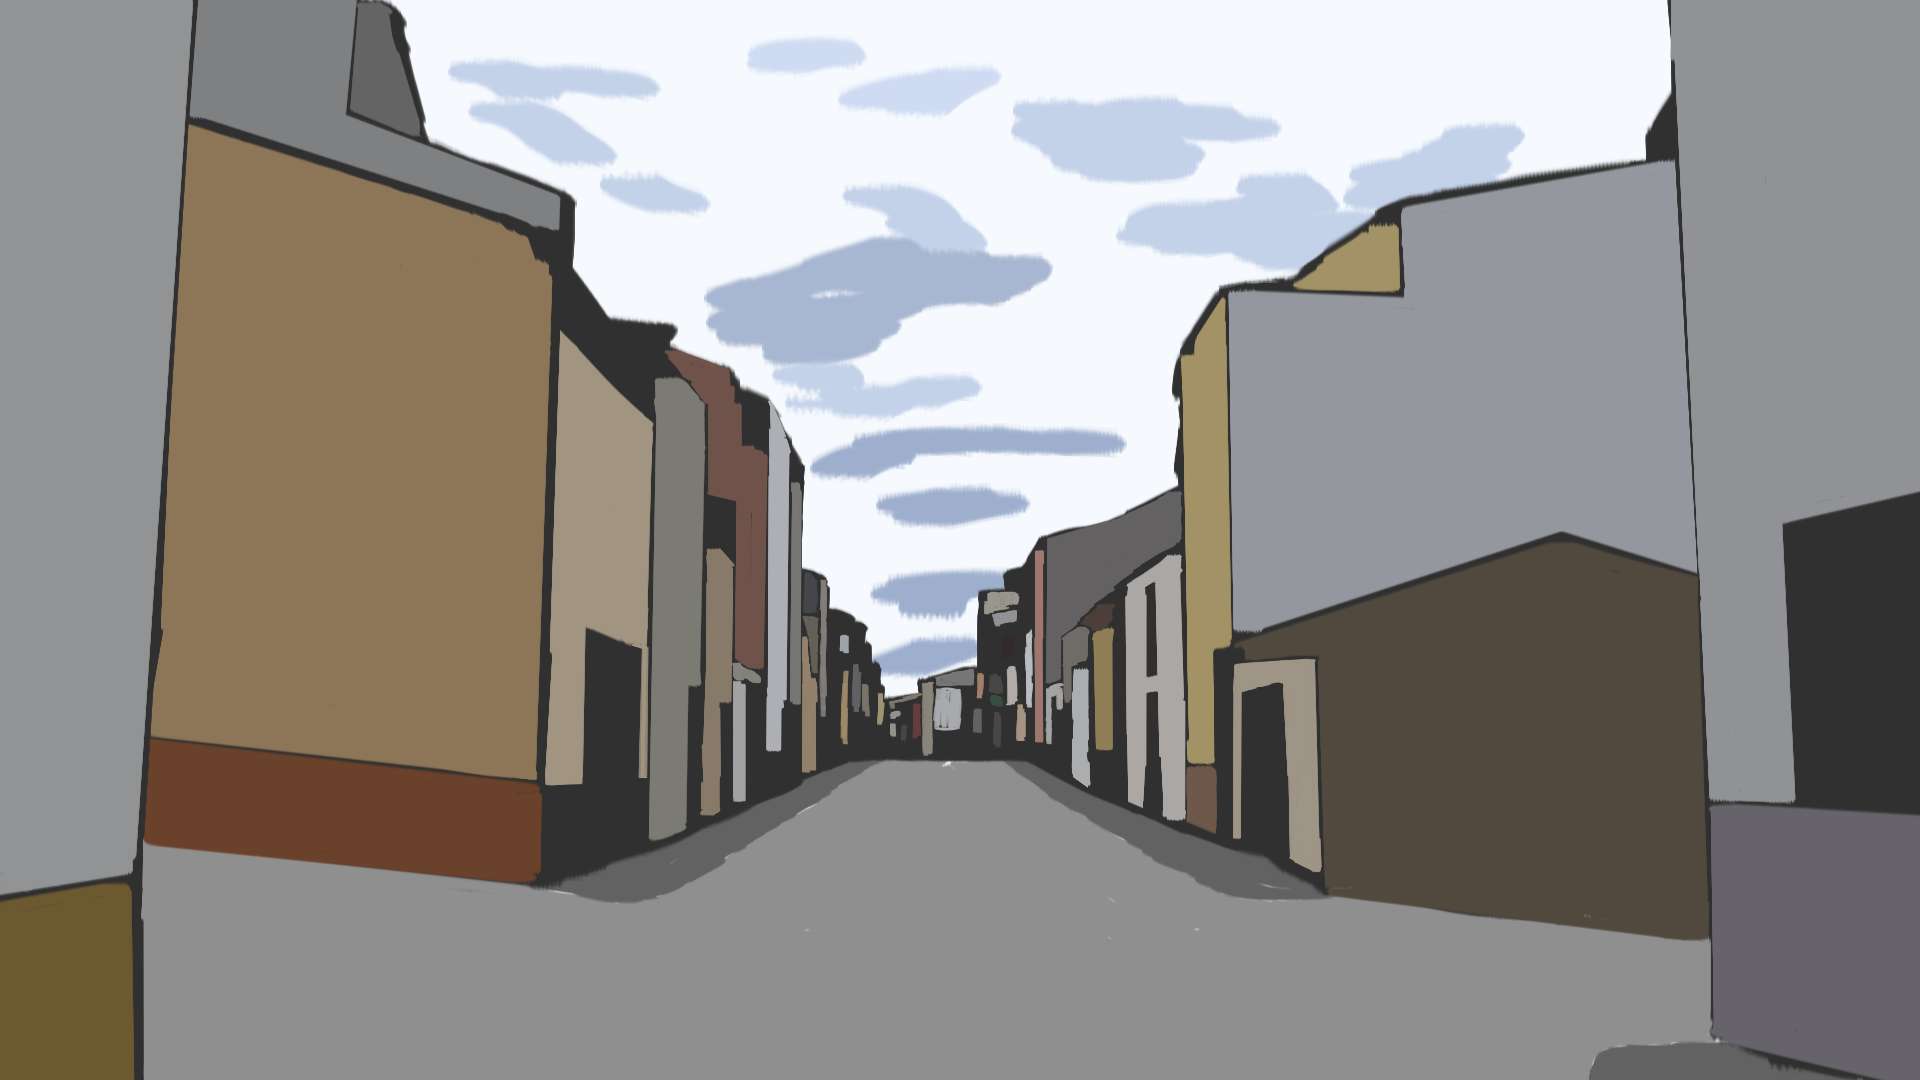
\includegraphics[width=\textwidth]{imgs/c_torre_2.png}
        \caption{Calle Torre: Boceto de la segunda sección}
        \label{fig:torre_boceto_2}
    \end{figure}
    \clearpage
    \begin{figure}[h!]
        \centering
        \includegraphics[width=\textwidth]{imgs/C_torre_foto_2.JPG}
        \caption{Calle Torre: Fotografía de la tercera sección}
        \label{fig:torre_foto_3}
    \end{figure}

    \begin{figure}[h!]
        \centering
        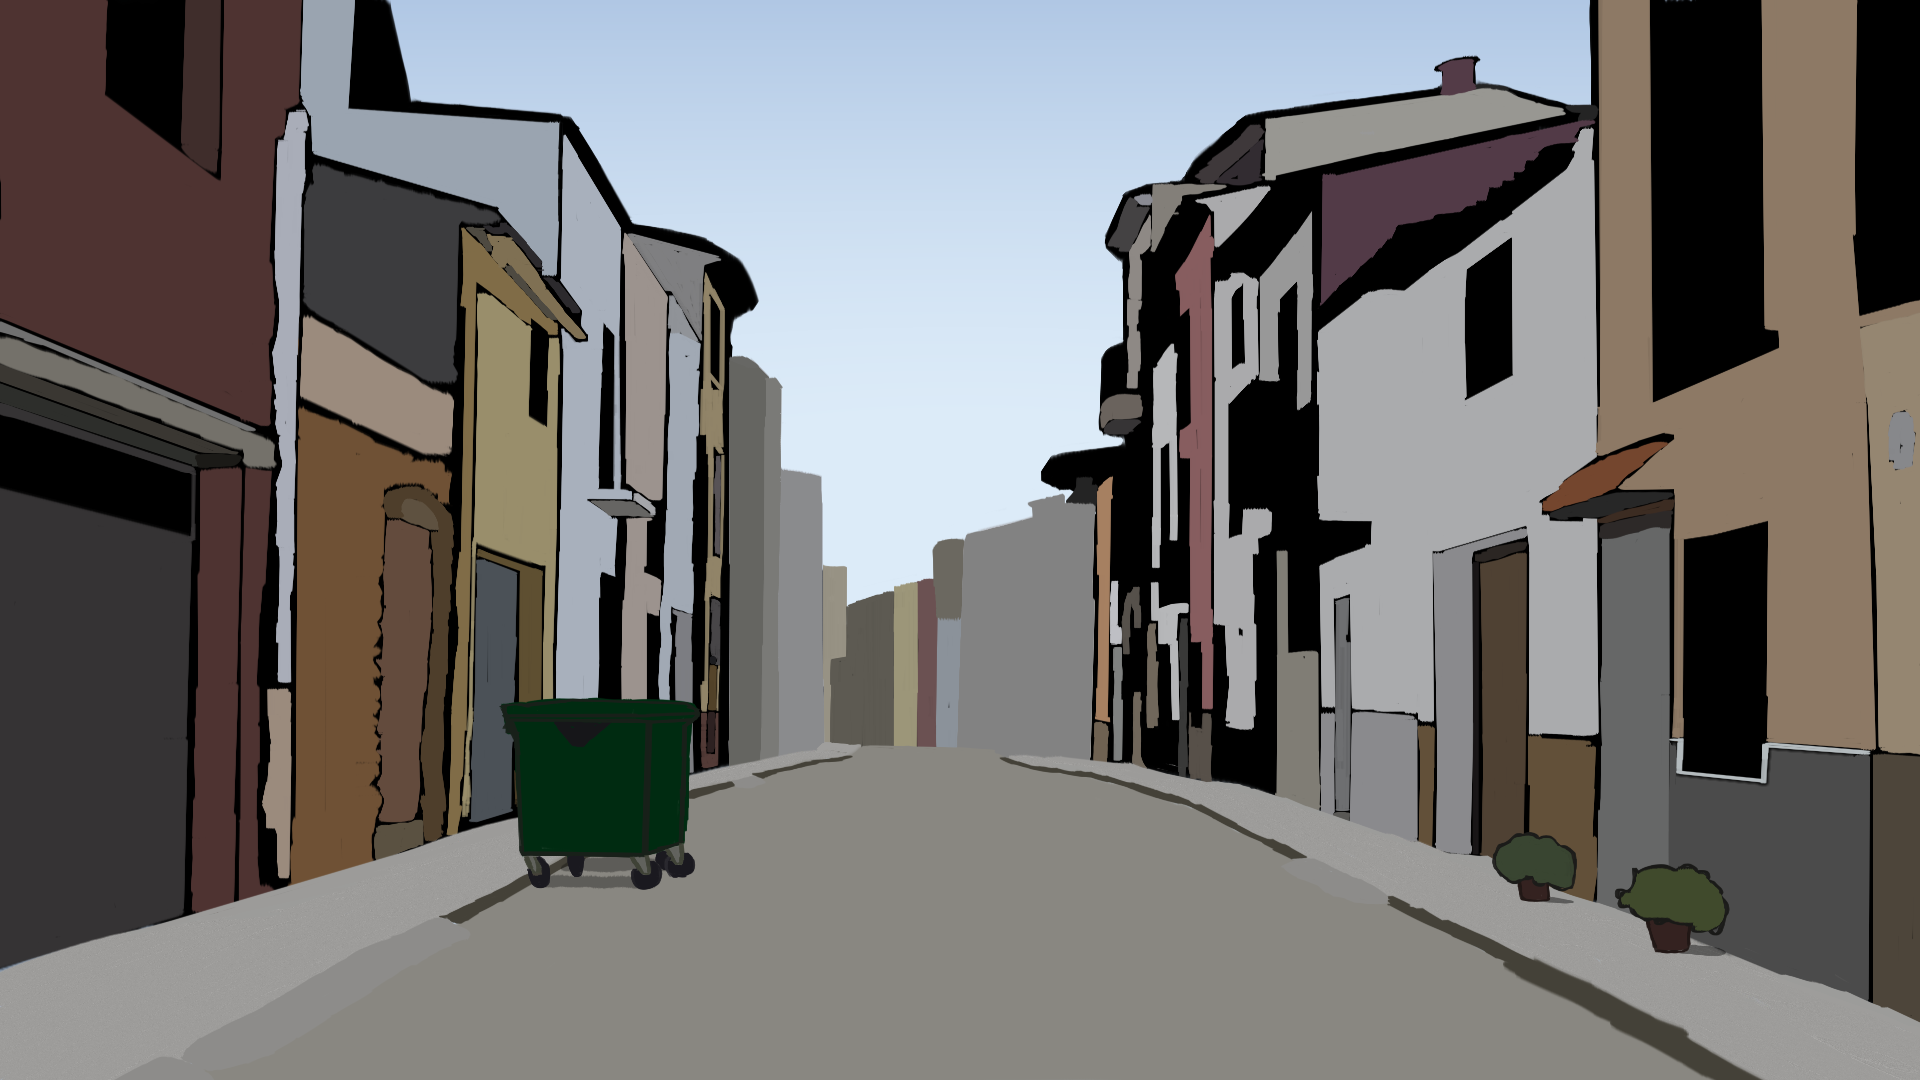
\includegraphics[width=\textwidth]{imgs/c_torre_3.png}
        \caption{Calle Torre: Boceto de la tercera sección}
        \label{fig:torre_boceto_3}
    \end{figure}
    \clearpage
    \begin{figure}[h!]
        \centering
        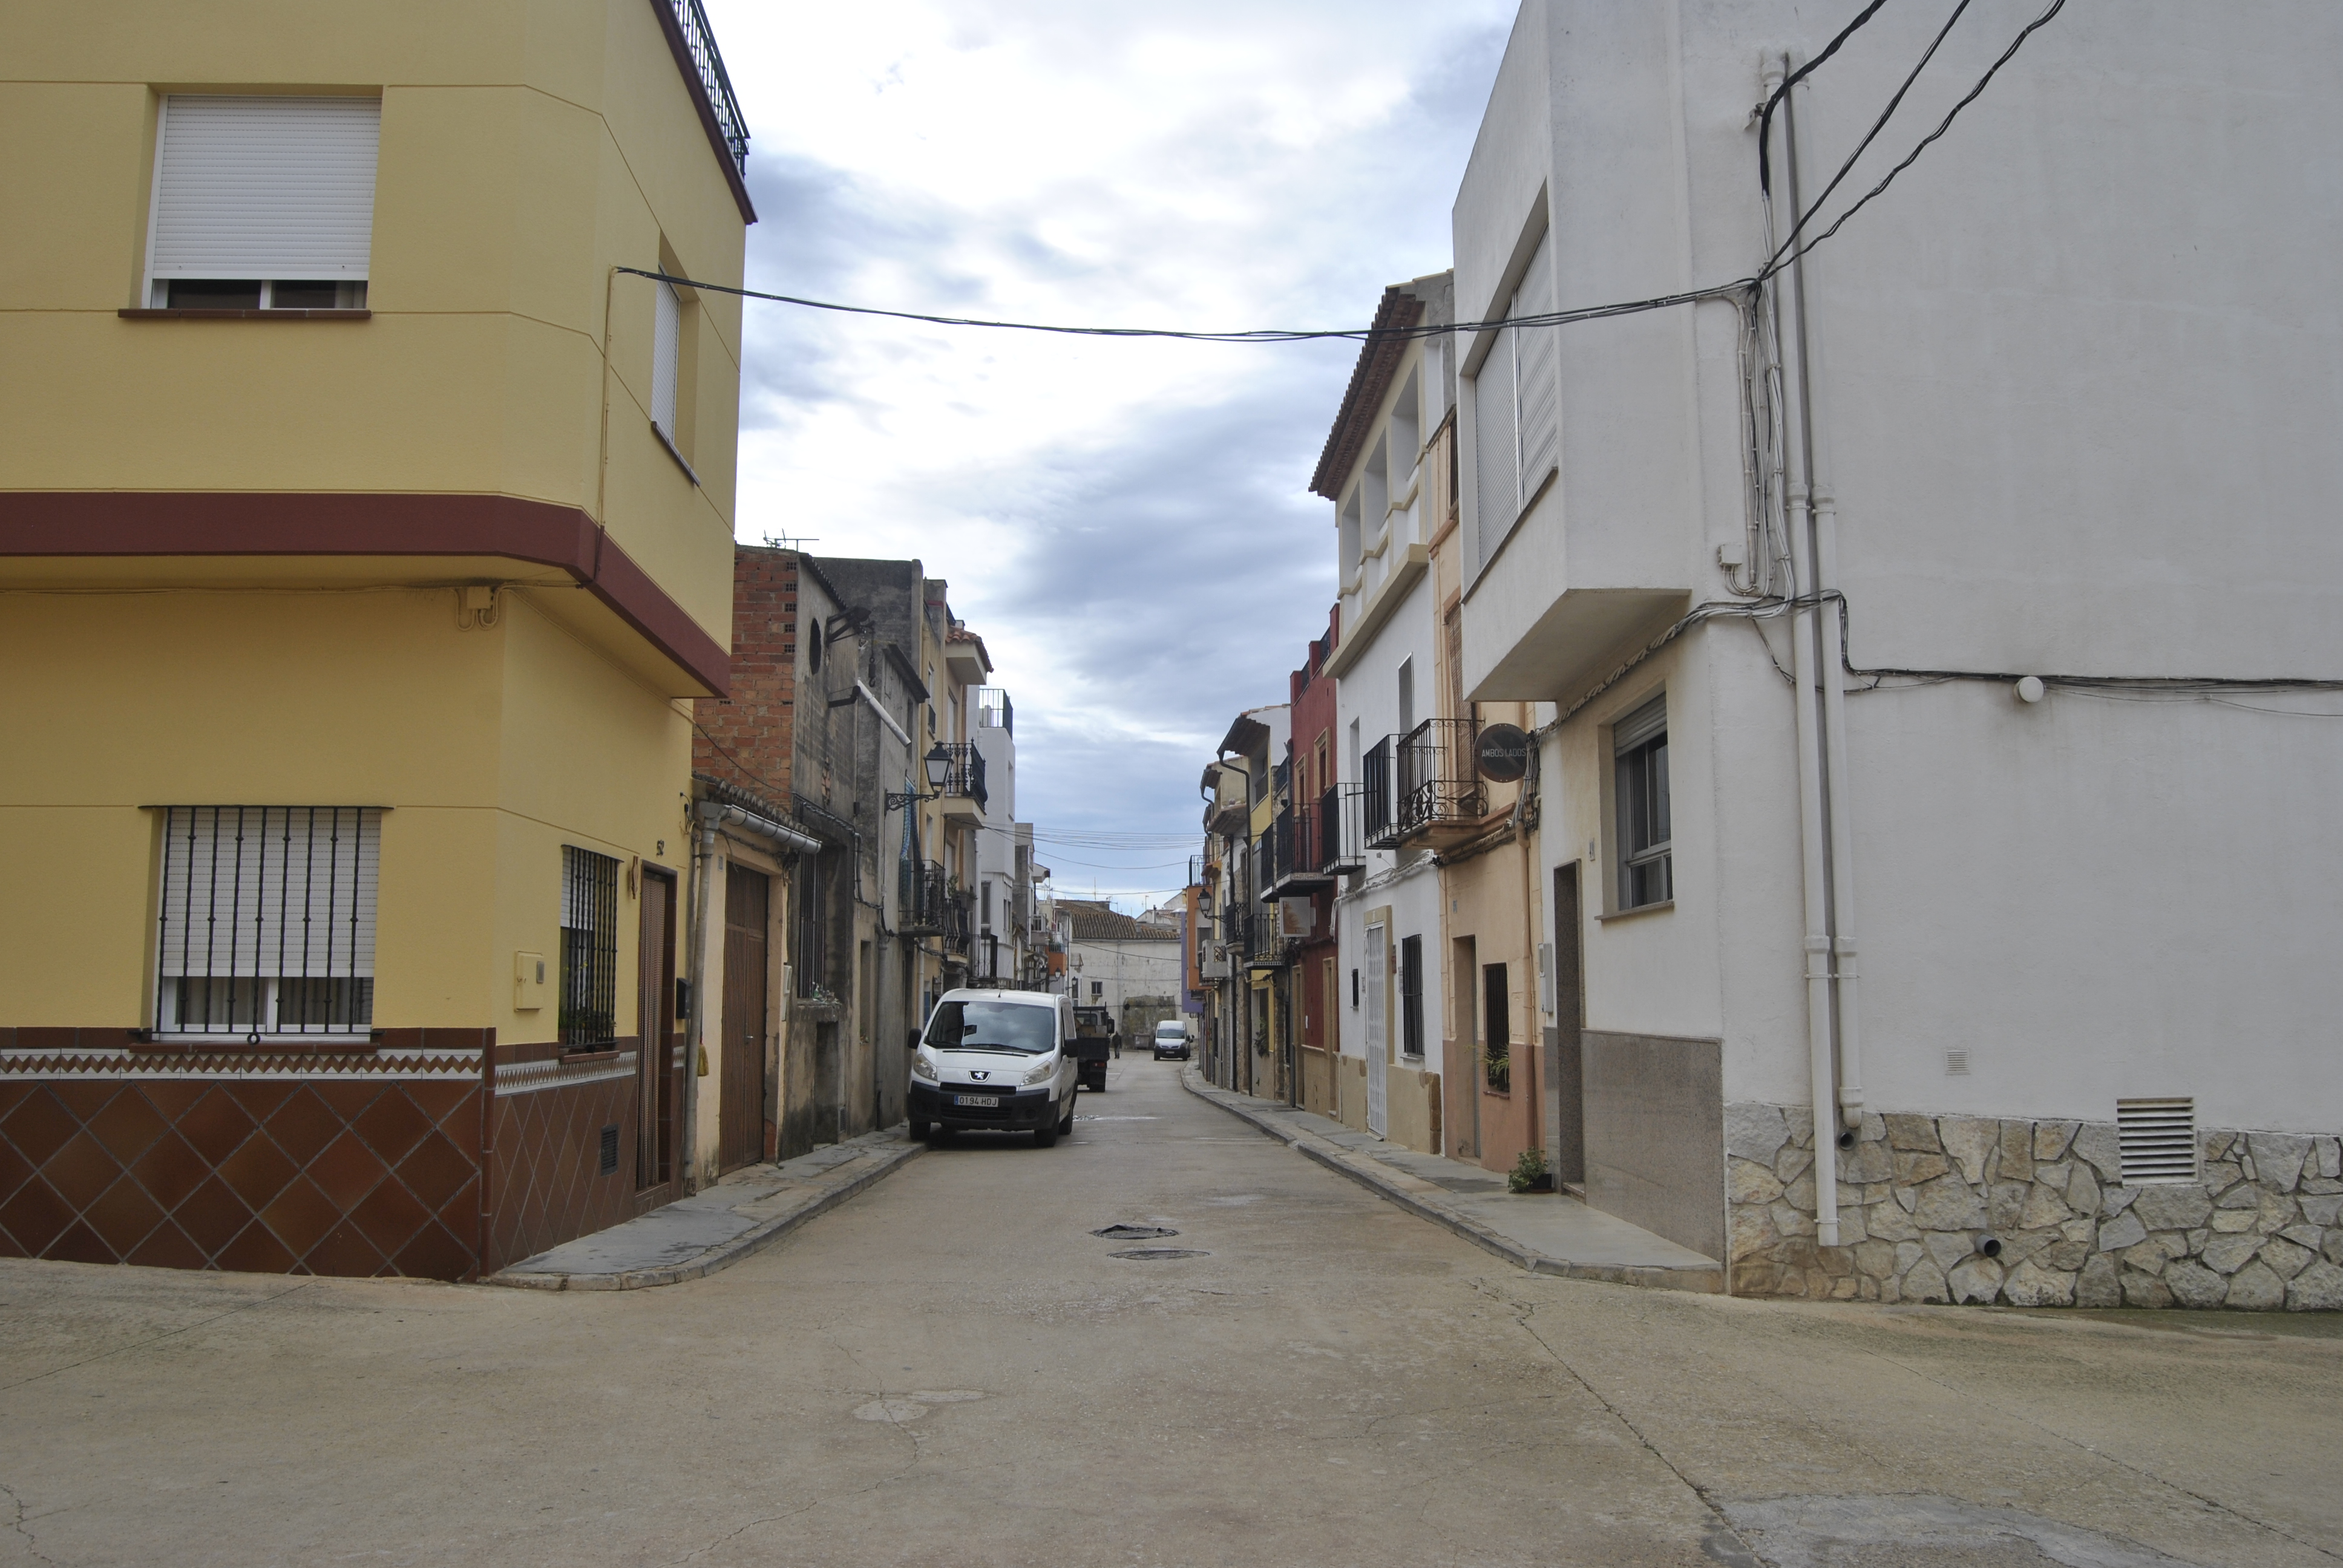
\includegraphics[width=\textwidth]{imgs/C_torre_foto_3.JPG}
        \caption{Calle Torre: Fotografía de la cuarta sección}
        \label{fig:torre_foto_4}
    \end{figure}

    \begin{figure}[h!]
        \centering
        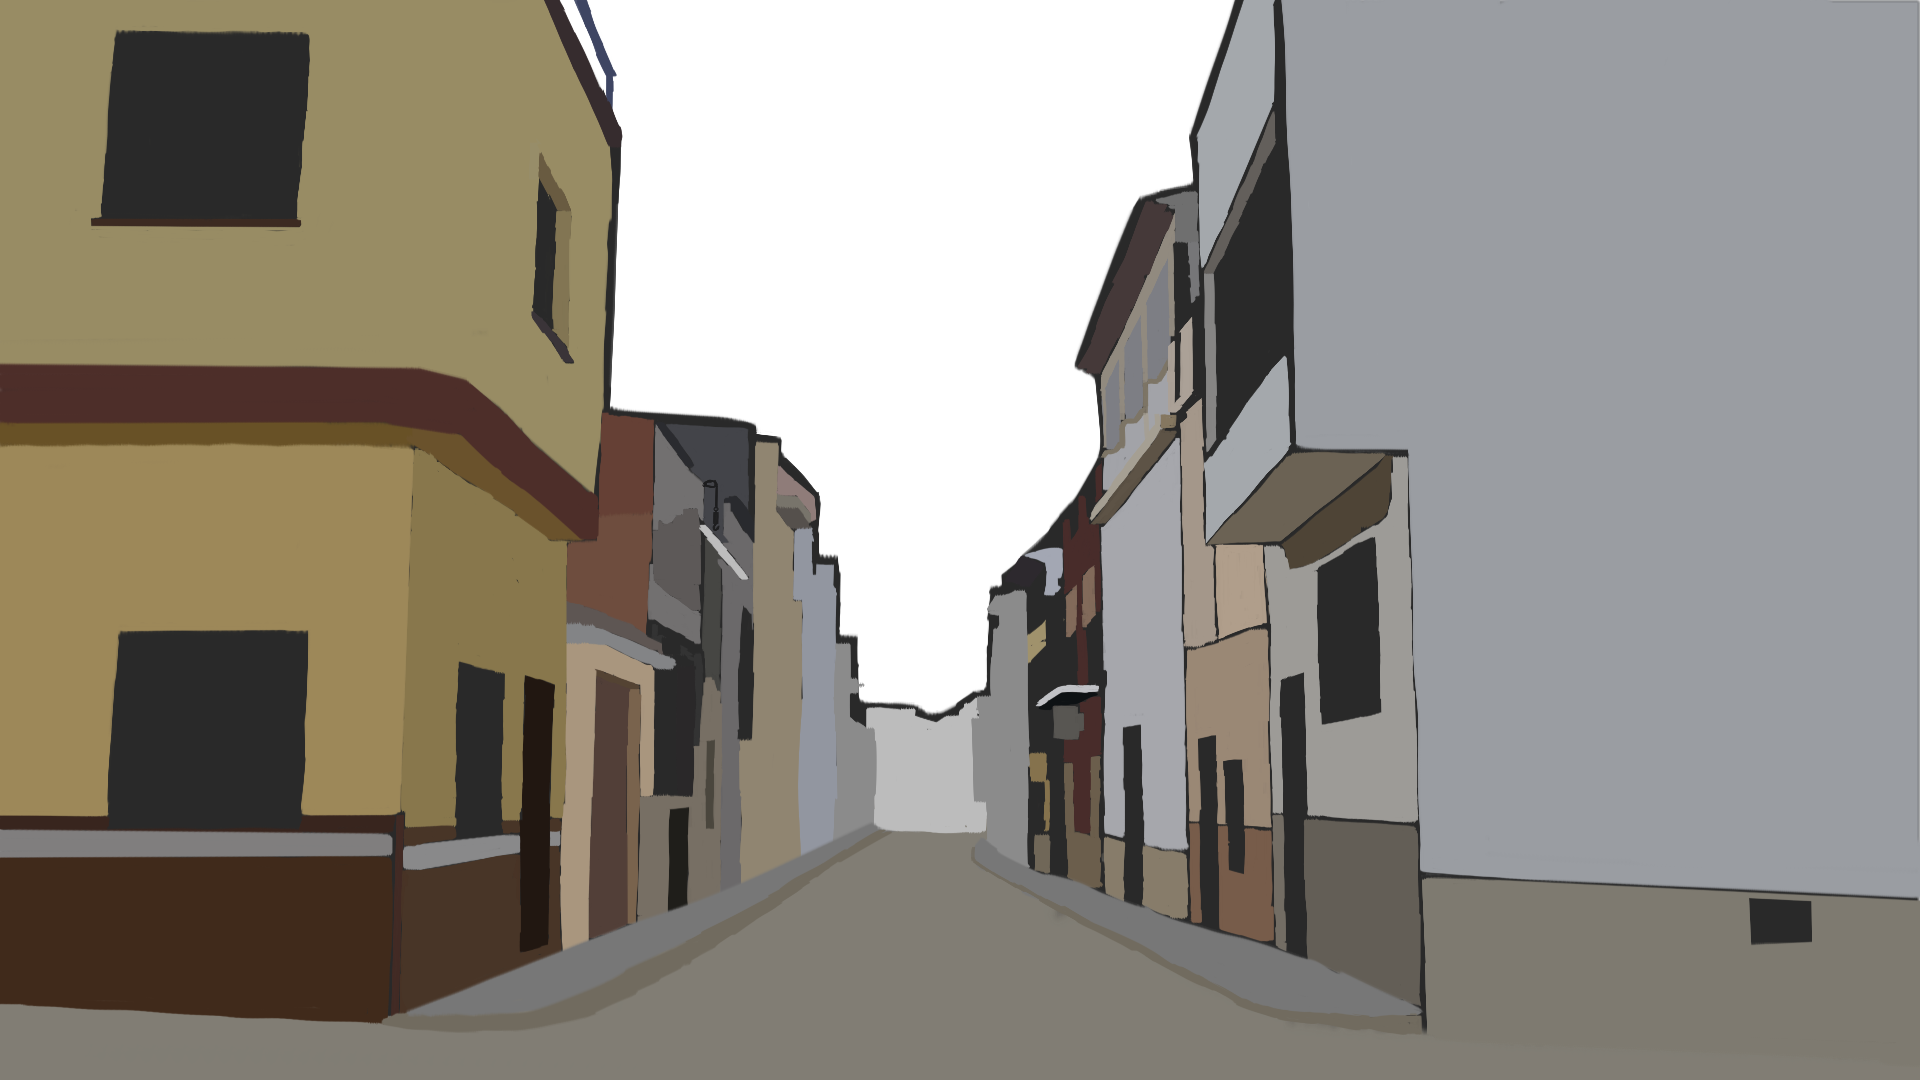
\includegraphics[width=\textwidth]{imgs/c_torre_4.png}
        \caption{Calle Torre: Boceto de la cuarta sección}
        \label{fig:torre_boceto_4}
    \end{figure}

    \clearpage

    \subsection{Calle Sant Antoni}
        Aunque mi parte de trabajo era dibujar la Calle Torre, a petición de Lucas, me pidió que dibujase la base de la Calle Sant Antoni para eliminar parte de su carga de trabajo.

        % Update Sant Antoni figure labels
        \begin{figure}[h!]
            \centering
            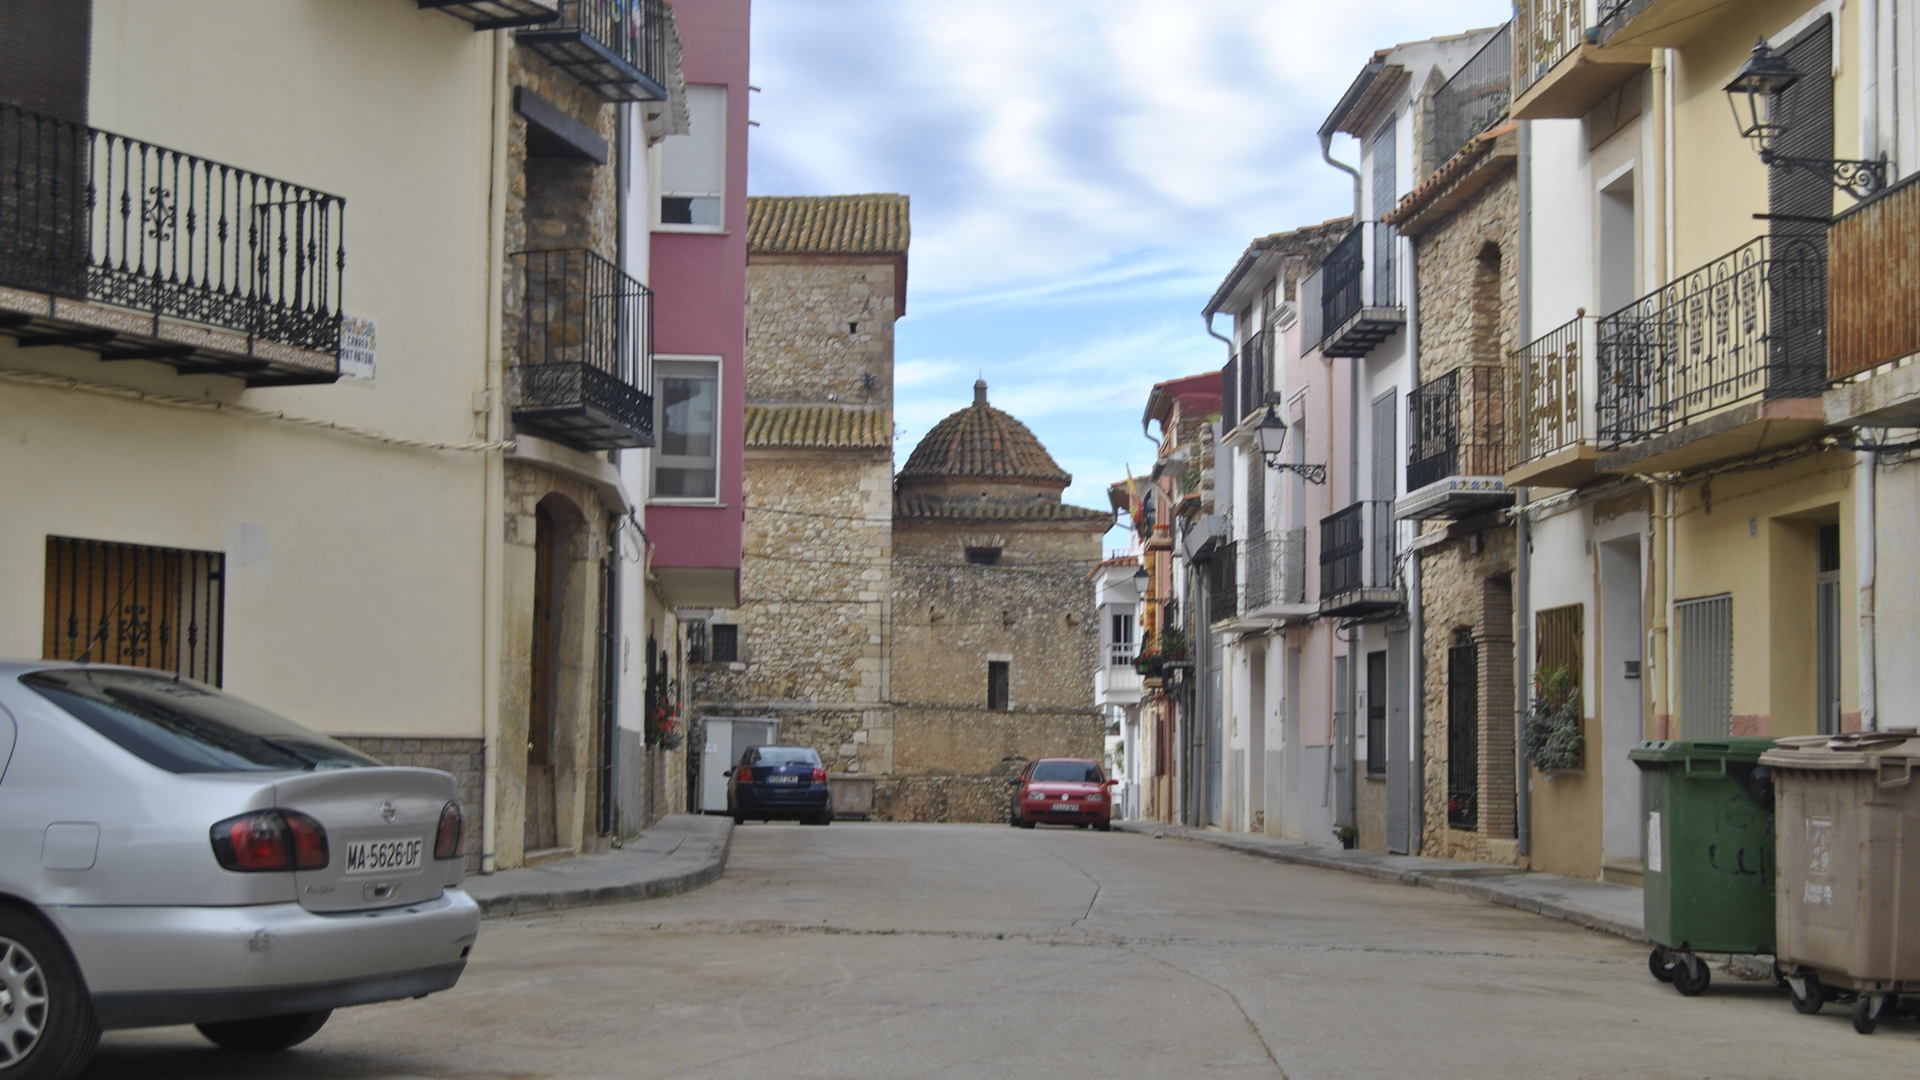
\includegraphics[width=\textwidth]{imgs/c_san_antoni_para_lucas_foto.png}
            \caption{Fotografía de la Calle Sant Antoni}
            \label{fig:santantoni_foto_1}
        \end{figure}

        \begin{figure}[h!]
            \centering
            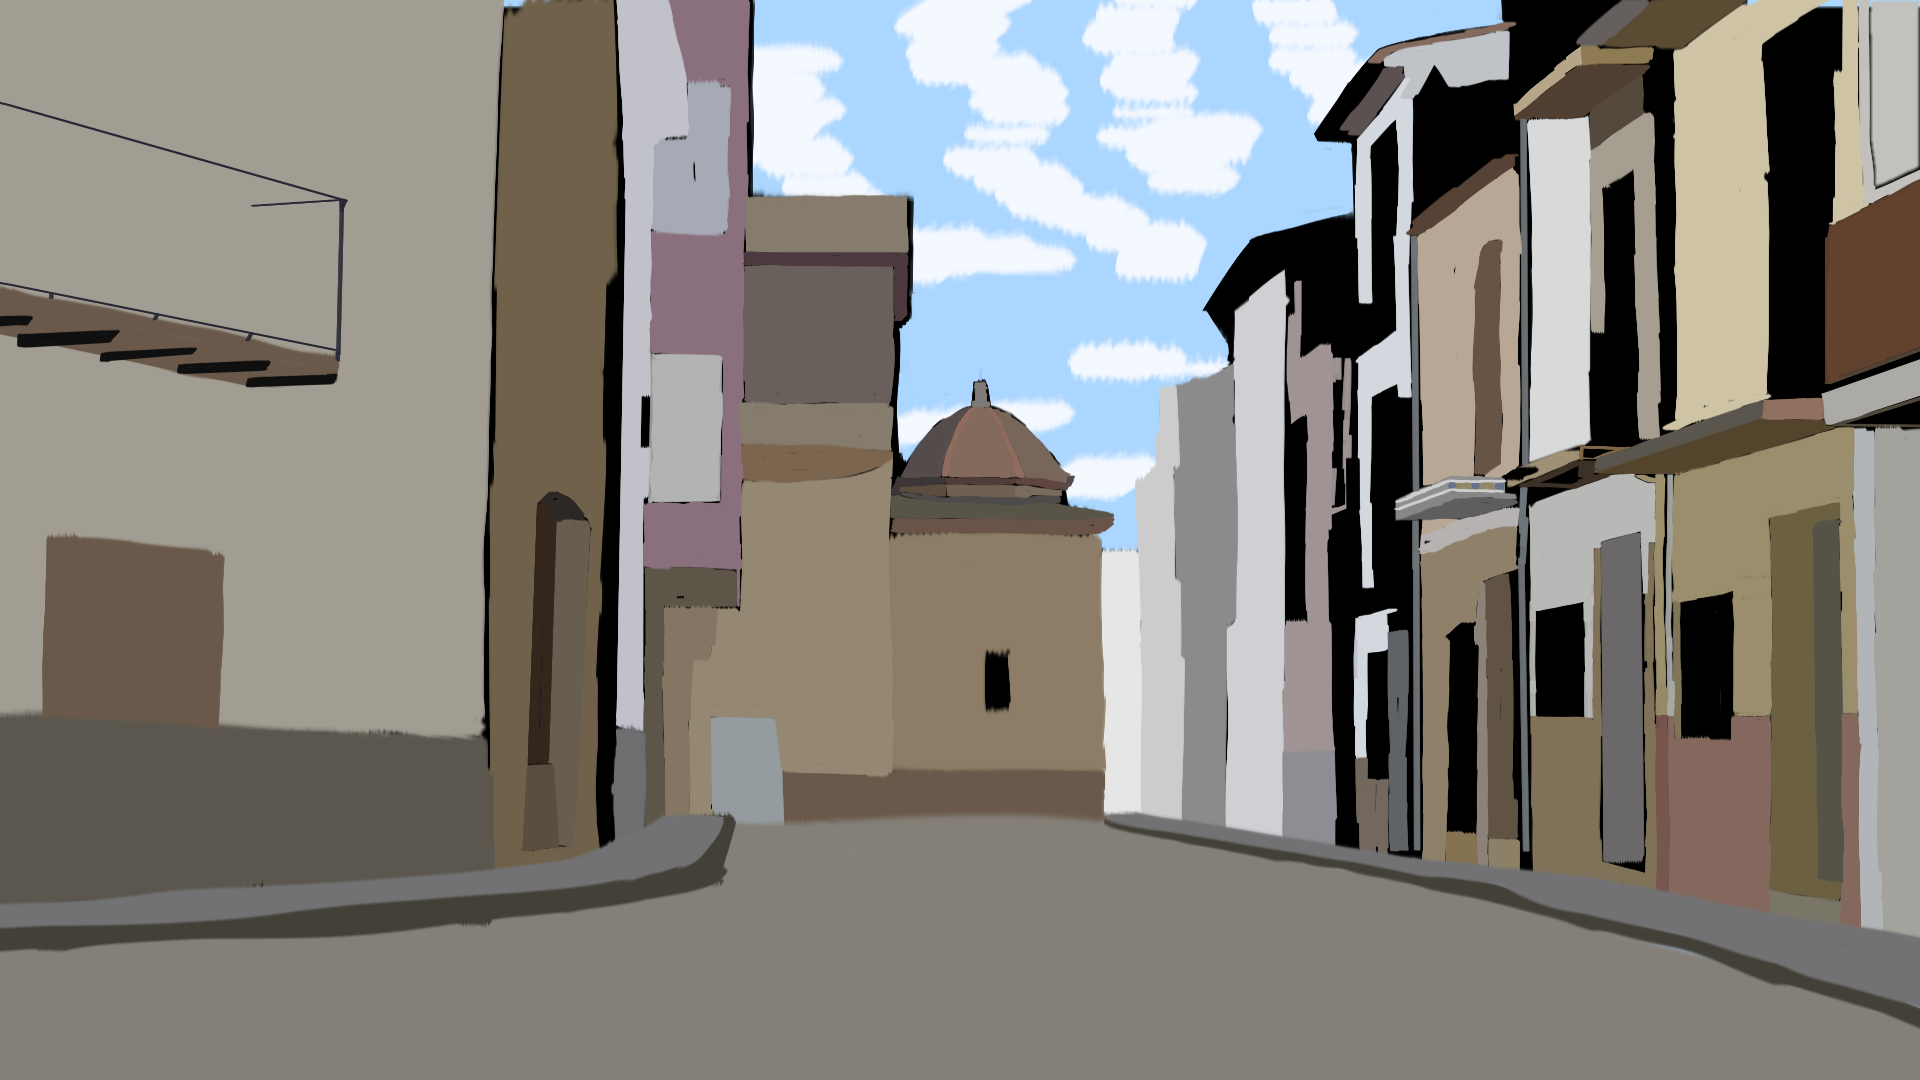
\includegraphics[width=\textwidth]{imgs/c_san_antoni_para_lucas.png}
            \caption{Boceto de la Calle Sant Antoni}
            \label{fig:santantoni_boceto_1}
        \end{figure}
    \newpage

\section{Diseño de interfaces}
    Aunque no directamente arte, diseñé algunas interfaces en Unity para el juego que íbamos a usar de forma común en todos los minijuegos.
    \begin{figure}[h!]
        \centering
        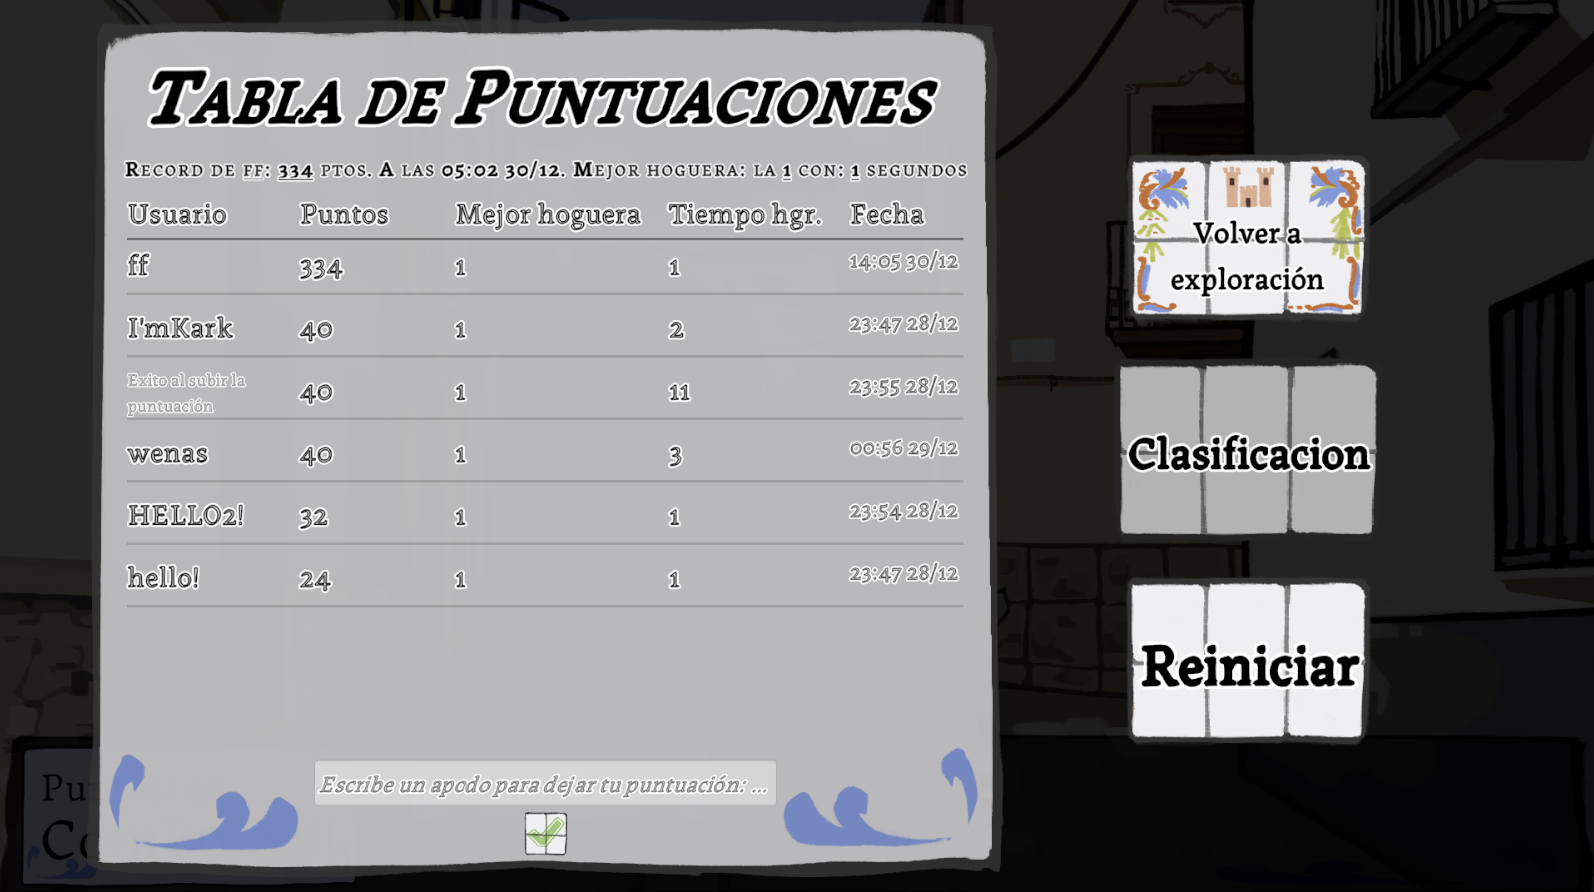
\includegraphics[width=0.8\textwidth]{imgs/leaderboard.png}
        \caption{Diseño general de la Tabla de Puntuaciones}
        \label{fig:diseno_tabla_puntuaciones}
    \end{figure}

    \begin{figure}[h!]
        \centering
        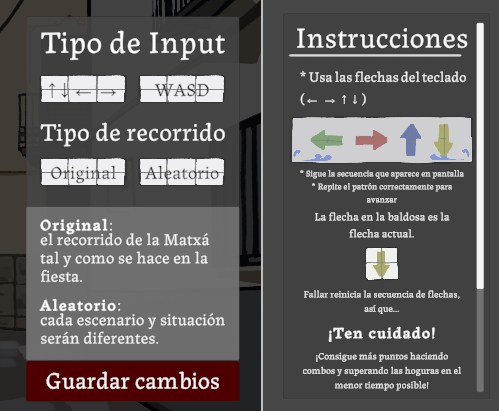
\includegraphics[width=0.8\textwidth]{imgs/common_panels.png}
        \caption{Diseño general de los paneles comunes}
        \label{fig:diseno_paneles_comunes}
    \end{figure}


\end{document}